\documentclass[a4paper,11pt]{article}

\usepackage[T1]{fontenc}
\usepackage[utf8]{inputenc}
% babel is broken on this system, using manual translations
\usepackage{geometry}
\geometry{margin=2.2cm}
\usepackage{booktabs}
\usepackage{longtable}
\usepackage{xcolor}
\usepackage{listings}
\usepackage{tikz}
\usetikzlibrary{arrows.meta,positioning,shapes.geometric}
\usepackage{hyperref}
\usepackage{float}

\renewcommand{\contentsname}{Inhaltsverzeichnis}
\renewcommand{\figurename}{Abbildung}
\renewcommand{\tablename}{Tabelle}

\lstdefinestyle{shared}{
  basicstyle=\ttfamily\small,
  keywordstyle=\color{blue!60!black},
  commentstyle=\color{green!40!black},
  stringstyle=\color{orange!60!black},
  numbers=left,
  numberstyle=\scriptsize\color{gray},
  stepnumber=1,
  numbersep=8pt,
  showstringspaces=false,
  breaklines=true,
  frame=single
}

\title{Technische Dokumentation des Chatbots\\
\large Datenanalyse auf Basis von KI-Methoden (WS 2022/2023)}
\author{Alwin, Andres, Donya, Luisa}
\date{4. M\"arz 2026}

\begin{document}
\maketitle
\tableofcontents
\newpage

\section{Zielsetzung}
Ziel des Projekts ist ein KI-gest\"utzter Mental-Health-Chatbot, der Nutzer bei Stress, Angst oder Schlafproblemen durch Check-ins und gezielte \"Ubungen (z.B. Atem\"ubungen, Grounding) unterst\"utzt.
Die Anwendung kombiniert eine Inferenz-Pipeline (Bag-of-Words + TFLearn) mit einem zustandsbehafteten Dialog-Manager und einer modernen Weboberfl\"ache.

Die Live-Demo ist unter \href{https://chatbot-mz6p.onrender.com/}{https://chatbot-mz6p.onrender.com/} erreichbar.

\section{System\"ubersicht}
\begin{itemize}
  \item \textbf{Backend:} Flask-App mit Textvorverarbeitung, Sentiment-Analyse (TextBlob) und zustandsbehafteter Logik.
  \item \textbf{Dialog-Manager:} Verwendet eine State-Machine (\texttt{transitions}) f\"ur gef\"uhrte \"Ubungen.
  \item \textbf{Modell:} TFLearn-Feedforward-Netz mit Softmax-Klassifikation.
  \item \textbf{Frontend:} Interaktive Oberfl\"ache mit Buttons, klickbaren Tipps und Animationen.
\end{itemize}

\section{Datei\"ubersicht}
\begin{longtable}{p{0.38\linewidth} p{0.55\linewidth}}
\toprule
\textbf{Datei} & \textbf{Funktion} \\
\midrule
\texttt{chatbot/app.py} & Flask-App mit Textverarbeitung, Modellinferenz und API-Routen. \\
\texttt{chatbot/chat.json} & Trainingsdaten: Intents, Beispiele und Antworten. \\
\texttt{chatbot/train.py} & Training-Skript zum Erzeugen von Modellartefakten. \\
\texttt{chatbot/dialogue\_manager.py} & Zustandsbehaftetes Dialog-Management und Sentiment-Analyse. \\
\texttt{chatbot/model.tflearn*} & Gespeichertes TFLearn-Modell (Weights + Meta). \\
\texttt{chatbot/trained\_data} & Gepickelte Trainingsdaten (Vokabular, Klassen, BoW-Arrays). \\
\texttt{chatbot/templates/index.html} & UI-Struktur mit interaktiven Buttons und klickbaren Tipps. \\
\texttt{chatbot/static/style.css} & Layout, Farbwelt und Animationen der Oberfl\"ache. \\
\texttt{render.yaml} & Render-Deployment (Build + Start Command). \\
\texttt{requirements.txt} & Python-Abh\"angigkeiten. \\
\bottomrule
\end{longtable}

\section{Backend: Modell und Antwortlogik}
\subsection{Textvorverarbeitung}
Die Eingabe wird tokenisiert, von Stoppw\"ortern bereinigt und mittels Snowball-Stemmer normalisiert. Daraus entsteht ein Bag-of-Words-Vektor, der den Modelleingang bildet.

\subsection{Inferenz-Pipeline}
\begin{figure}[H]
\centering
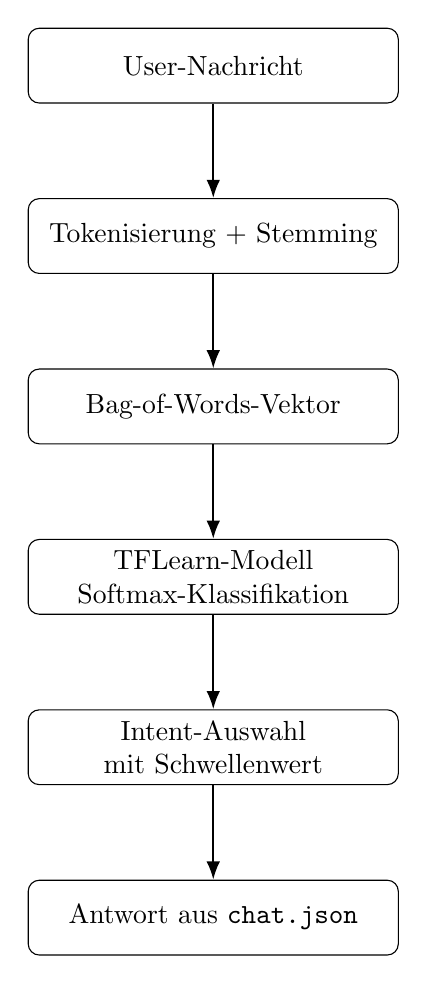
\begin{tikzpicture}[
  node distance=1.2cm and 1.6cm,
  block/.style={rectangle, draw, rounded corners, align=center, minimum width=4.7cm, minimum height=0.95cm},
  line/.style={-Latex, thick}
]
\node[block] (input) {User-Nachricht};
\node[block, below=of input] (token) {Tokenisierung + Stemming};
\node[block, below=of token] (bow) {Bag-of-Words-Vektor};
\node[block, below=of bow] (model) {TFLearn-Modell\\Softmax-Klassifikation};
\node[block, below=of model] (intent) {Intent-Auswahl\\mit Schwellenwert};
\node[block, below=of intent] (answer) {Antwort aus \texttt{chat.json}};

\draw[line] (input) -- (token);
\draw[line] (token) -- (bow);
\draw[line] (bow) -- (model);
\draw[line] (model) -- (intent);
\draw[line] (intent) -- (answer);
\end{tikzpicture}
\caption{Datenfluss der Antwortgenerierung.}
\end{figure}

\subsection{Antwortauswahl}
Die Softmax-Ergebnisse werden nach Wahrscheinlichkeit sortiert. Unterhalb eines Schwellenwerts werden Intents verworfen.
Die erste passende Intent-Antwort aus \texttt{chat.json} wird zuf\"allig ausgew\"ahlt. Bei Unsicherheit erfolgt eine Standardantwort.

\section{Frontend}
\subsection{UI-Konzept}
Die Oberfl\"ache ist bewusst kompakt gehalten: Kopfbereich mit Projektkontext, darunter ein Chatfenster mit
Message-Bubbles und ein Eingabefeld. Ein Typing-Indikator signalisiert aktive Verarbeitung.

\subsection{Client-Ablauf}
\begin{itemize}
  \item Nutzertext wird direkt als Benutzer-Nachricht gerendert.
  \item Ein Fetch-Request sendet \texttt{msg} an \texttt{/get}.
  \item Die Serverantwort wird als Bot-Nachricht eingef\"ugt.
\end{itemize}

\section{Verbesserungen}
\begin{itemize}
  \item Sentiment-Analyse zur empathischen Einleitung von Antworten.
  \item Gef\"uhrte, interaktive \"Ubungen (z.B. Box-Breathing) mittels State-Machine.
  \item Benutzeroberfl\"ache mit klickbaren Tipps und Schnellwahl-Buttons.
  \item Robuste Modellinitialisierung und Health-Endpoint.
  \item Explizites Deaktivieren von Eager-Execution f\"ur stabile Inferenz.
  \item Besseres Request-Handling im Frontend mit Typing-Indikator und Fehler-Feedback.
\end{itemize}

\section{Ausf\"uhrung und Tests}
\subsection{Live Demo}
Die Anwendung kann ohne lokale Installation direkt im Browser getestet werden: \\
\href{https://chatbot-mz6p.onrender.com/}{https://chatbot-mz6p.onrender.com/}

\subsection{Lokales Starten}
Voraussetzung: Python 3.10 und eine virtuelle Umgebung.
\begin{lstlisting}[style=shared,language=bash]
python -m venv .venv
source .venv/bin/activate
pip install -r requirements.txt
python -m nltk.downloader punkt stopwords -d chatbot/nltk_data
python chatbot/app.py
\end{lstlisting}
Anschlie\ss end die Anwendung unter \texttt{http://localhost:5000} aufrufen.

\subsection{Test: /get Endpoint}
Ein einfacher Unit-Test pr\"uft, ob der \texttt{/get}-Endpoint auf eine Nachricht reagiert:
\begin{lstlisting}[style=shared,language=bash]
.venv/bin/python -m unittest tests.test_get
\end{lstlisting}

\section{Codeauszug (Python)}
\begin{lstlisting}[style=shared,language=Python]
@app.route("/get", methods=["POST"])
def chatbot_response():
    msg = request.form.get("msg", "")
    state = session.get("chat_state", {})
    res, intent = bot.get_response(msg, state)
    final_response = res or DEFAULT_RESPONSE
    session["chat_state"] = state
    return jsonify(final_response)
\end{lstlisting}

\section{Codeauszug (JavaScript)}
\begin{lstlisting}[style=shared]
const response = await fetch(endpoint, {
  method: "POST",
  headers: { "Content-Type": "application/x-www-form-urlencoded;charset=UTF-8" },
  body: new URLSearchParams({ msg: rawText }),
});
const data = await response.json();
const botMsg = data.text || "Keine Antwort vom Server.";
appendMessage("bot", botMsg);
\end{lstlisting}

\end{document}
